\subsection{Frontend}\label{subsec:frontend_design}
The frontend of Drive-LaB has two responsibilities in the overall system, namely collection and presentation of location data. As the interface for users, it is designed with ease of use and understandability in mind. Given the non-trivial responsibilities, these requirements pose significant design challenges. These are addressed in Sections \ref{subsubsec:design_datacollection} and \label{subsubsec:design_datapresentation}.

\subsubsection{Data Collection}\label{subsubsec:design_datacollection}
Data collection is complicated by requiring user interaction. Without additional hardware, it is not possible to automatically detect the beginning or end of a trip. As such, users are required to manually control when their smartphone should start and stop tracking their movement.
Upon ending a trip, a sequence of actions takes place. A series of locations has been logged, and is passed on to the API server. To achieve this, data is converted into classes readable by the API server. Furthermore, trips are packaged into JSON objects which can be received by the REST service hosted on the API server described in Section \ref{sec:api_server}. If the API server is unavailable, trips are cached locally and bundled the next time a trip is ended. This sequence of events does not require user interaction, and is fully automatable. Summarizing the process of collecting location data, one can gather three different working states for the application:

\begin{itemize}
\item Idle - Ready to track a new trip
\item Tracking - Continually logging new positions
\item Finishing up - Packaging and sending all logged data
\end{itemize}

These working states are made visible through a central button in the application, as seen in Figure \ref{fig:start_stop_finishing_trip}. The progression of working states happens from left to right. "START TUR" (START TRIP) means the application is ready to track a new trip, and invites the user to do so. "STOP TUR" (STOP TRIP) means the application is currently tracking, and invites the user to end the trip when finished. Finally the user is presented with a message, "AFSLUTTER TUR" (FINISHING TRIP), informing the user that the tracking has stopped, but the application is still working. Upon finishing the process of sending the trip to the API server, the application will once again be ready to start a new trip, displaying "START TUR" for the user.
While the logic behind the button is complex, usage is simple and easy to understand. The user only have to define the beginning and end of a trip; the application takes care of the rest.

\begin{figure}[tb]
\centering
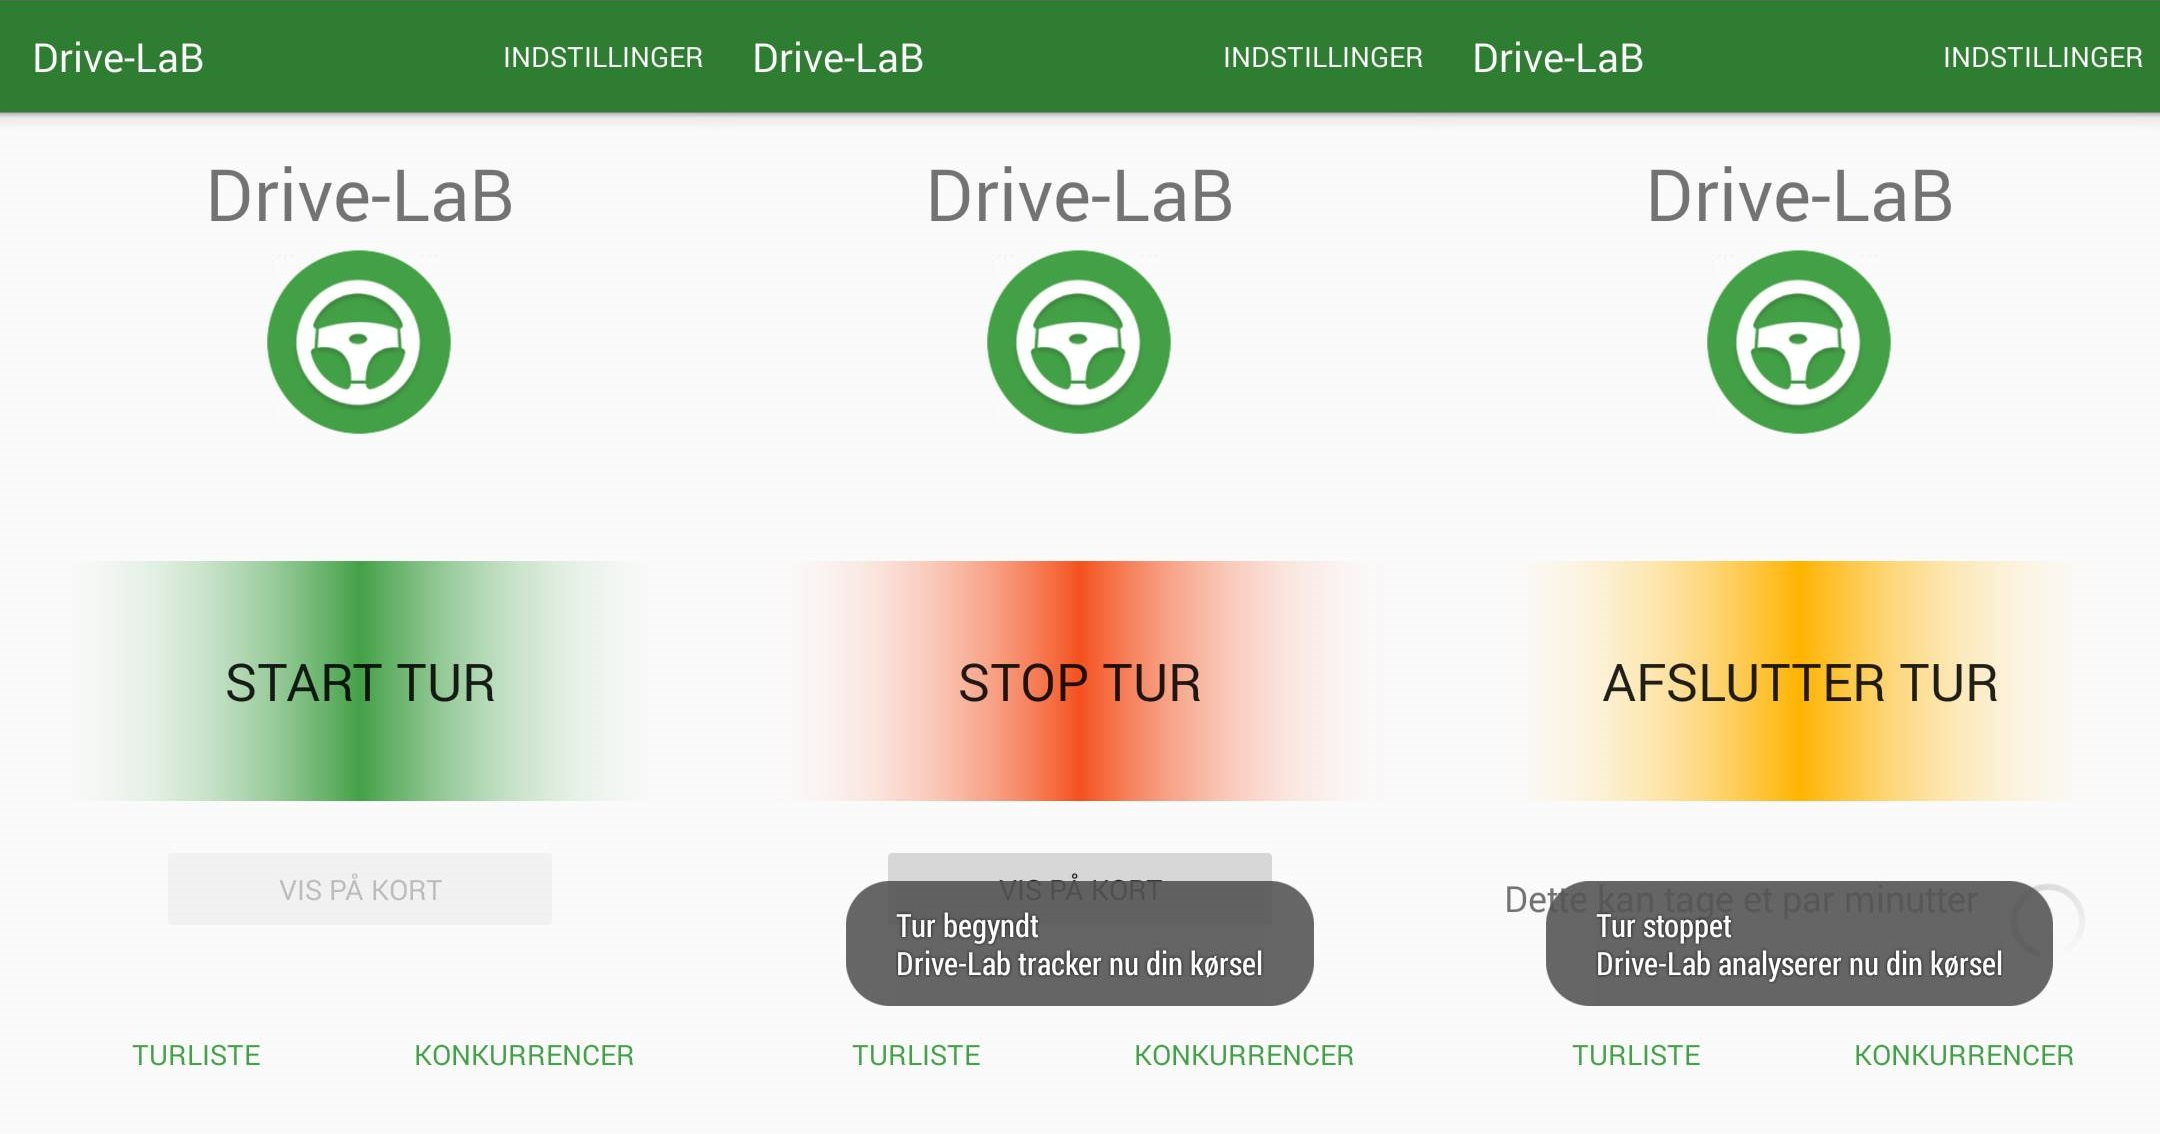
\includegraphics[width=0.465\textwidth]{Pictures/start_stop_finishing_trip}
\caption{Design of the Start/Stop/Finishing button}
\label{fig:start_stop_finishing_trip}
\end{figure}

\subsubsection{Data Presentation} \label{subsubsec:design_datapresentation}
Data presentation is complicated, both by the extensiveness of the data itself, but also the limited screen size of a smartphone. In other words, the application has to fit a lot of information into a small screen. With the goal of having an easily understandable system, the extensive data is simplified by presenting descriptive summaries, rather than raw data. The small screen is however still a challenge, and for this reason the application offers a multilevel description of trips, each presenting a certain level of data. Each level of description is presented on its own screen, and ranges from a broad description down to specific statistics. For an arbitrary trip, these screens can be seen in Figure \ref{fig:tripoverview}.

\begin{figure}[tb]
\centering
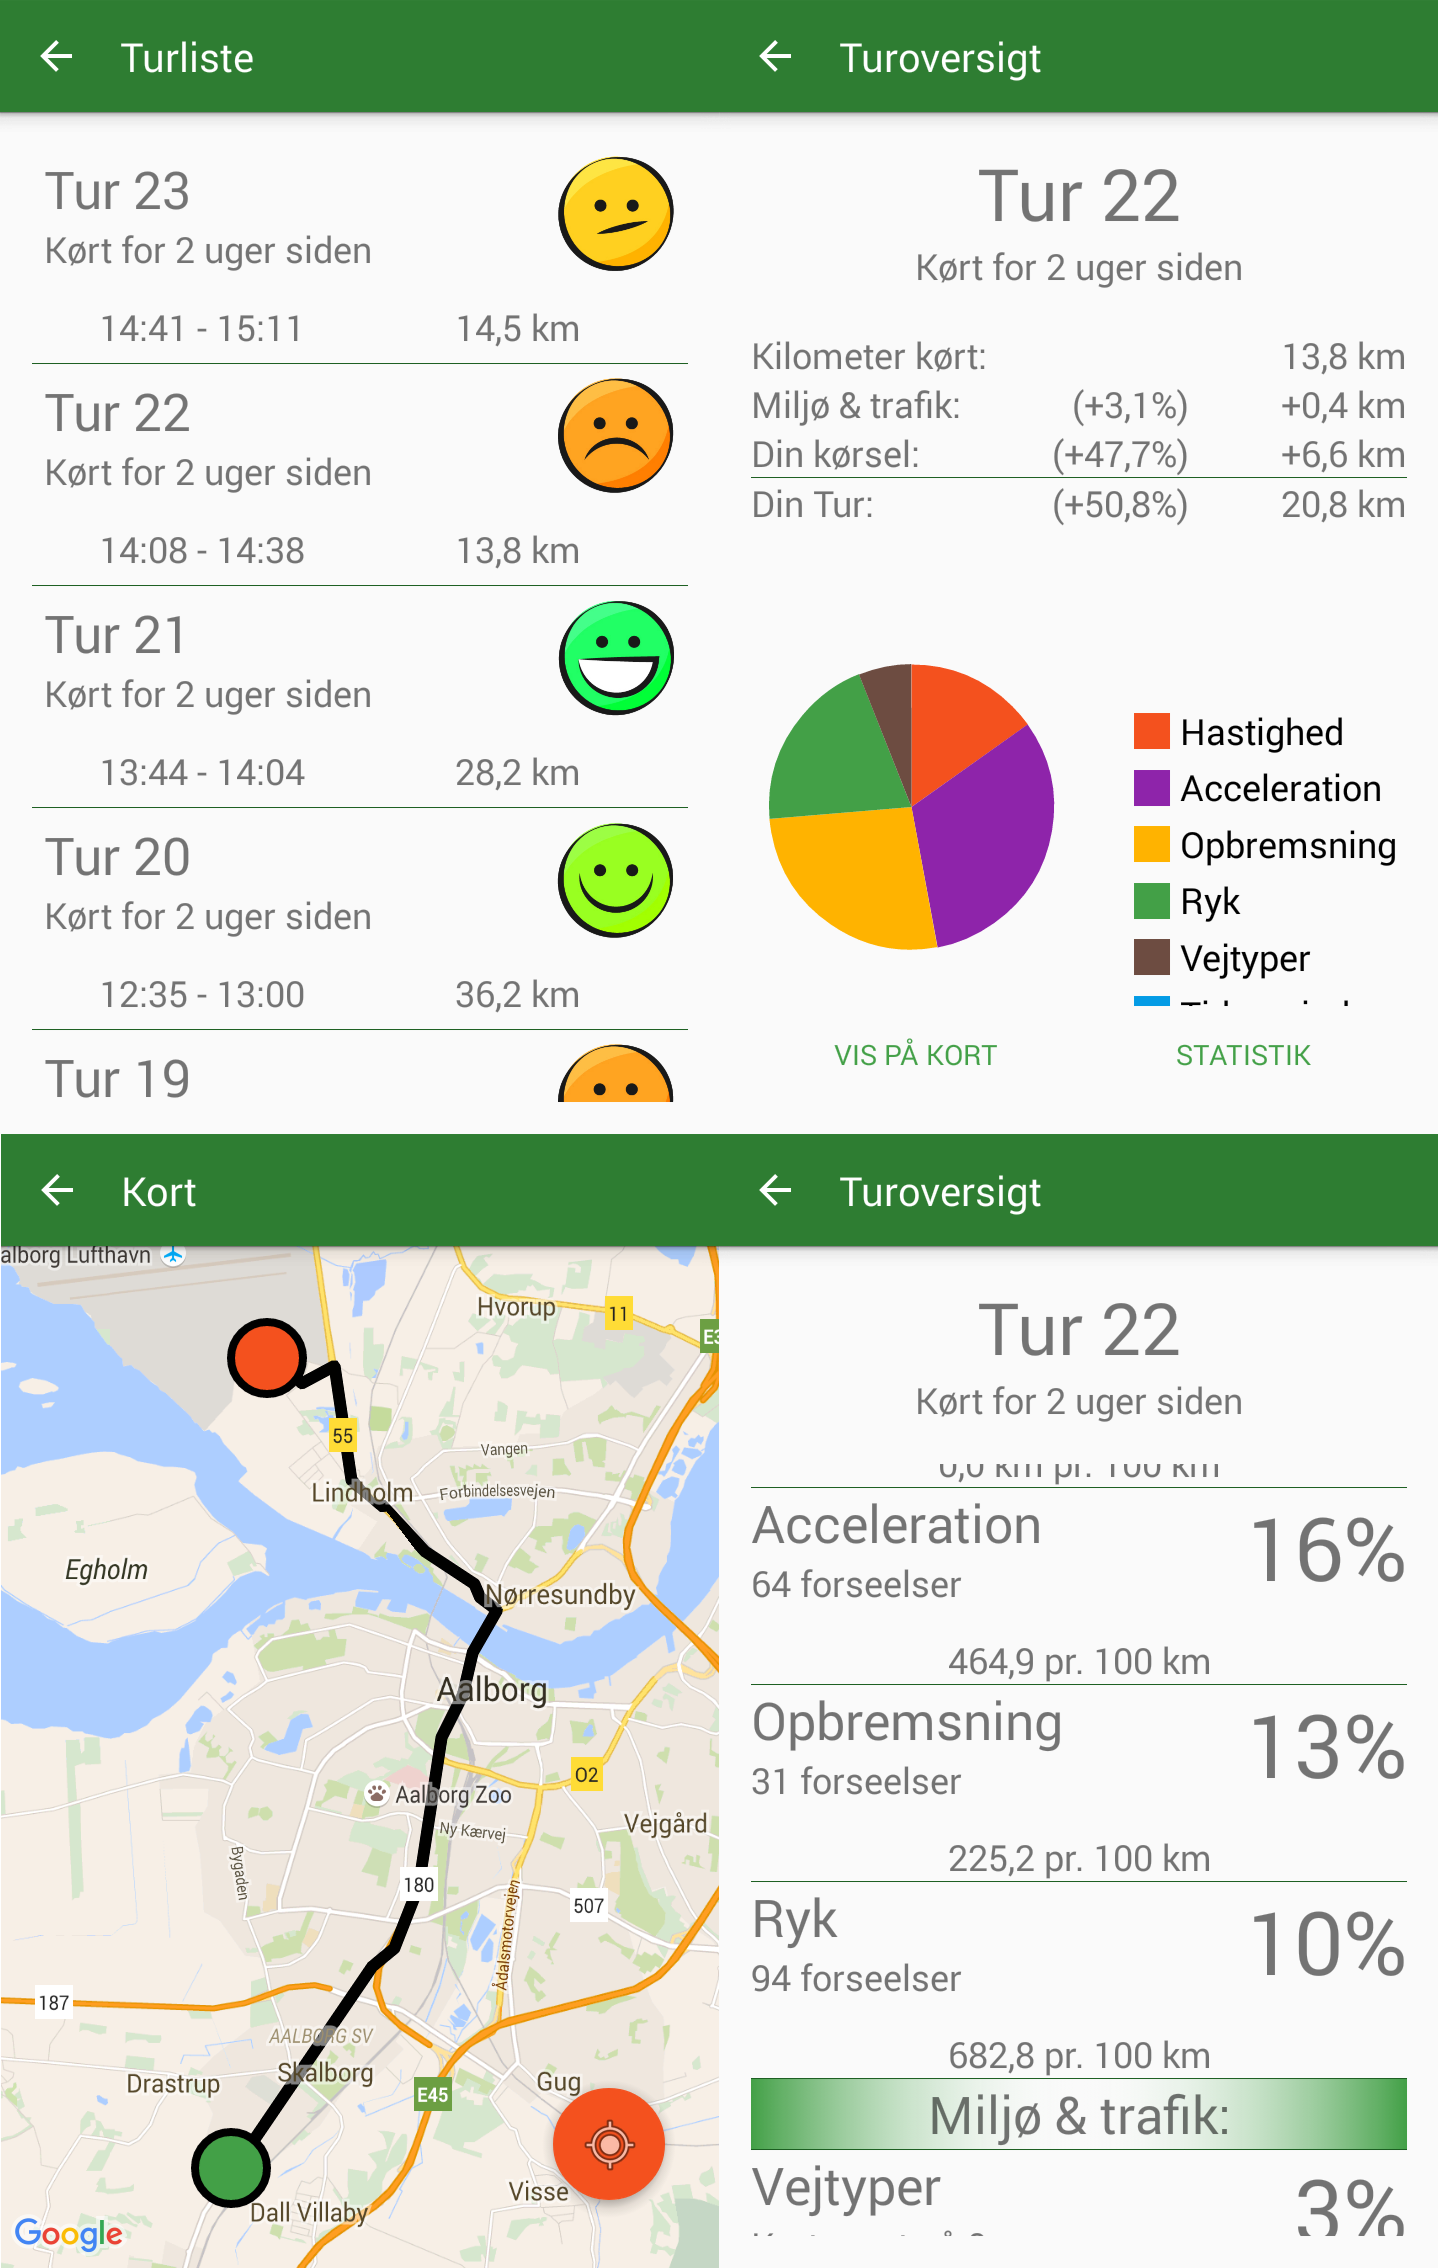
\includegraphics[width=0.465\textwidth]{Pictures/tripoverview}
\caption{Presentation of trips split across 4 screens}
\label{fig:tripoverview}
\end{figure}

On the top left screen, users are first presented with a list their trips ordered by date. For each trip, general statistics are displayed. These are useful mostly for identifying the trip. In key with keeping Drive-LaB simple to use and understand, the user can also see the trip score summarized as a smiley. Smileys range between green/happy and red/sad. They allow for cursory trip evaluation, without the need to look at more detailed statistics.
The top right screen is shown when clicking a trip, and displays a more extensive score summary. The screen uses a pie chart to visualize the relative influence of each metric, allowing the user to identify points of possible improval.
On Figure \ref{fig:tripoverview}, the bottom screens both show evaluation specifics, letting the user see exactly what was registered during a trip. The left screen places the route on top of a map, showing the user exactly where locations were logged. The right screen shows exact metric counts, allowing the user to see why a metric score turned out the way it did.
The different levels of information allow users to navigate only to the desired detail level. As such, some users might be satisfied with seeing the resulting smiley, and will not be forced to look at details. For those who want more detailed results however, these are also made available.

\subsubsection{Competitions} \label{subsubsec:competitions}
Drive-LaB is designed to offer competitions as an additional service, both for the insurance company and end users. Competitions allow the insurance company to collect additional data about users. For users, bringing a competitive element into Drive-LaB can act as incentive to use it and perform to ones best ability. In the Drive-LaB application, users are able to browse active competitions and choose which to participate in. Section \ref{subsec:userexp} further describes end user experiments supported by a competition hosted within Drive-LaB. When participating in a competition, the user gains access to live statistics for the duration of the competition. These include current ranking and a leaderboard meant to encourage and motivate users to perform better.